\documentclass[10pt]{article}
\usepackage{amsmath,amsfonts,times}
\usepackage{graphicx,color,tikz,pgfplots}
\usepackage[paperwidth=14.5cm,paperheight=4.6cm,lmargin=0in,rmargin=0in,tmargin=0.in,bmargin=0.in]{geometry}
\usepackage{bm}
\usetikzlibrary{arrows,shadings,shapes.arrows,decorations.pathreplacing,calc, positioning}
\usepgfplotslibrary{fillbetween}

\pgfplotsset{
  compat=newest
}

\newlength{\dx}
\setlength{\dx}{1.5cm}

\newlength{\circleRadius}
\setlength{\circleRadius}{0.95\dx}

\definecolor{outside}{rgb}{0, 1, 0}
\definecolor{cutcell}{rgb}{0, 0.5, 1}
\definecolor{inside}{rgb}{1, 0, 0}

\tikzset{
  edge/.style={thick, draw=black},
  tree/.style={thick, draw=black, densely dotted},
  bvh/.style={draw=black, minimum width=5mm, minimum height=5mm, rectangle, very thick},
  vertex/.style={circle, inner sep=0pt, minimum width=4pt, draw=black, fill=black, node contents={}},
  point/.style={circle, inner sep=0pt, minimum width=6pt, thick, draw=black, fill=white},
  root/.style={ultra thick, densely dashed, draw=black},
  left/.style={very thick, draw=black, solid, fill=blue, fill opacity=0.2},
  right/.style={very thick, draw=black, solid, fill=red, fill opacity=0.2},
}

\begin{document}
\centering
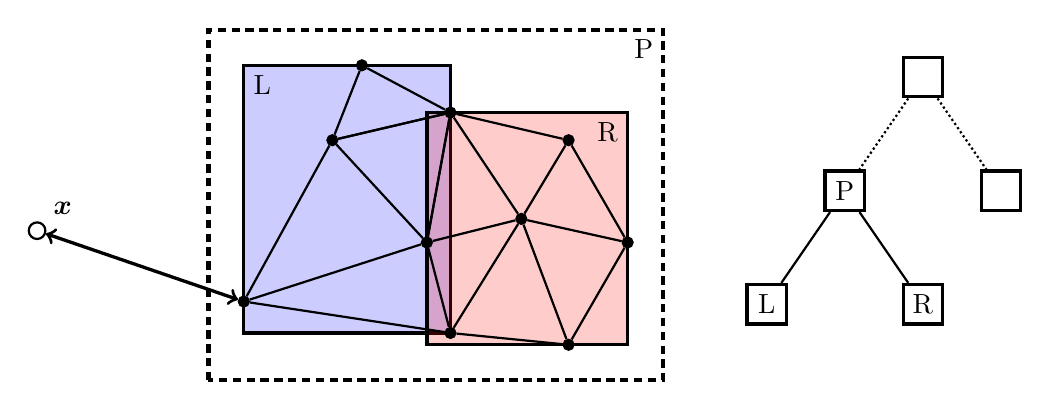
\begin{tikzpicture}

    \draw[root] (-2.55\dx,-1.166\dx) rectangle (1.3\dx, 1.8\dx);
    \draw[left] (-2.25\dx,-0.766\dx) rectangle (-0.5\dx, 1.5\dx);
    \draw[right] (-0.7\dx,-0.866\dx) rectangle (1\dx, 1.1\dx);
    
    \node (v0) at (0.1\dx,0.2\dx) [vertex];
    \node (v1) at (\dx, 0) [vertex];
    \node (v2) at (0.5\dx, 0.866\dx) [vertex];
    \node (v3) at (-0.5\dx, 1.1\dx) [vertex];
    \node (v4) at (-0.7\dx, 0) [vertex];
    \node (v5) at (-0.5\dx, -0.766\dx) [vertex];
    \node (v6) at (0.5\dx, -0.866\dx) [vertex];

    \node (v7) at (-1.5\dx, 0.866\dx) [vertex];
    \node (v8) at (-1.25\dx, 1.5\dx) [vertex];
    \node (v9) at (-2.25\dx, -0.5\dx) [vertex];

    \draw[edge] (v0)--(v1);
    \draw[edge] (v0)--(v2);
    \draw[edge] (v0)--(v3);
    \draw[edge] (v0)--(v4);
    \draw[edge] (v0)--(v5);
    \draw[edge] (v0)--(v6);

    \draw[edge] (v1)--(v2)--(v3)--(v4)--(v5)--(v6)--(v1);

    \draw[edge] (v3)--(v8)--(v7)--(v3);
    \draw[edge] (v4)--(v7)--(v3)--(v4);
    \draw[edge] (v9)--(v4);
    \draw[edge] (v9)--(v5);
    \draw[edge] (v9)--(v7);

    \node[bvh, alias=ROOT] at (3.5\dx, 1.4\dx) {};
    \node[bvh, alias=subtree, below right=0.6\dx and 0.3\dx of ROOT] {};
    \node[bvh, alias=P, below left=0.6\dx and 0.3\dx of ROOT] {P};
    \node[bvh, alias=L, below left=0.6\dx and 0.3\dx of P] {L};
    \node[bvh, alias=R, below right=0.6\dx and 0.3\dx of P] {R};

    \node[anchor=north east] at (1.3\dx, 1.8\dx) {P};
    \node[anchor=north west] at (-2.25\dx,1.5\dx) {L};
    \node[anchor=north east] at (\dx, 1.1\dx) {R};

    \draw[edge] (P) -- (L);
    \draw[edge] (P) -- (R);
    \draw[tree] (ROOT) -- (P);
    \draw[tree] (ROOT) -- (subtree);

    \node[point, alias=x] at (-4\dx, 0.1\dx) {};
    \node[anchor=south west] at (x.north east) {$\bm{x}$};
    \draw[very thick, <->] (x) -- (v9);

  
\end{tikzpicture}

\end{document} 
